%========================================
% DETAILED SOLUTIONS: Sistema de Coordenadas
%========================================

\subsection*{Ejercicio 1: Identificación de Cuadrantes}

\textbf{Problema 1:} $(5, 3)$

Como ambas coordenadas son positivas ($x > 0$ y $y > 0$), el punto se encuentra en el \textbf{Cuadrante I}.

\medskip

\textbf{Problema 2:} $(-2, 7)$

La coordenada $x$ es negativa ($x < 0$) y la coordenada $y$ es positiva ($y > 0$), por lo tanto el punto se encuentra en el \textbf{Cuadrante II}.

\medskip

\textbf{Problema 3:} $(-4, -6)$

Como ambas coordenadas son negativas ($x < 0$ y $y < 0$), el punto se encuentra en el \textbf{Cuadrante III}.

\medskip

\textbf{Problema 4:} $(8, -3)$

La coordenada $x$ es positiva ($x > 0$) y la coordenada $y$ es negativa ($y < 0$), por lo tanto el punto se encuentra en el \textbf{Cuadrante IV}.

\medskip

\textbf{Problema 5:} $(0, -5)$

Como la coordenada $x = 0$, el punto está sobre el \textbf{eje $y$}. Los puntos sobre los ejes no pertenecen a ningún cuadrante.

\medskip

\textbf{Problema 6:} $(6, 0)$

Como la coordenada $y = 0$, el punto está sobre el \textbf{eje $x$}. Los puntos sobre los ejes no pertenecen a ningún cuadrante.

\newpage

\subsection*{Ejercicio 2: Graficar Puntos}

Los puntos se grafican en el plano cartesiano de la siguiente manera:

\begin{center}
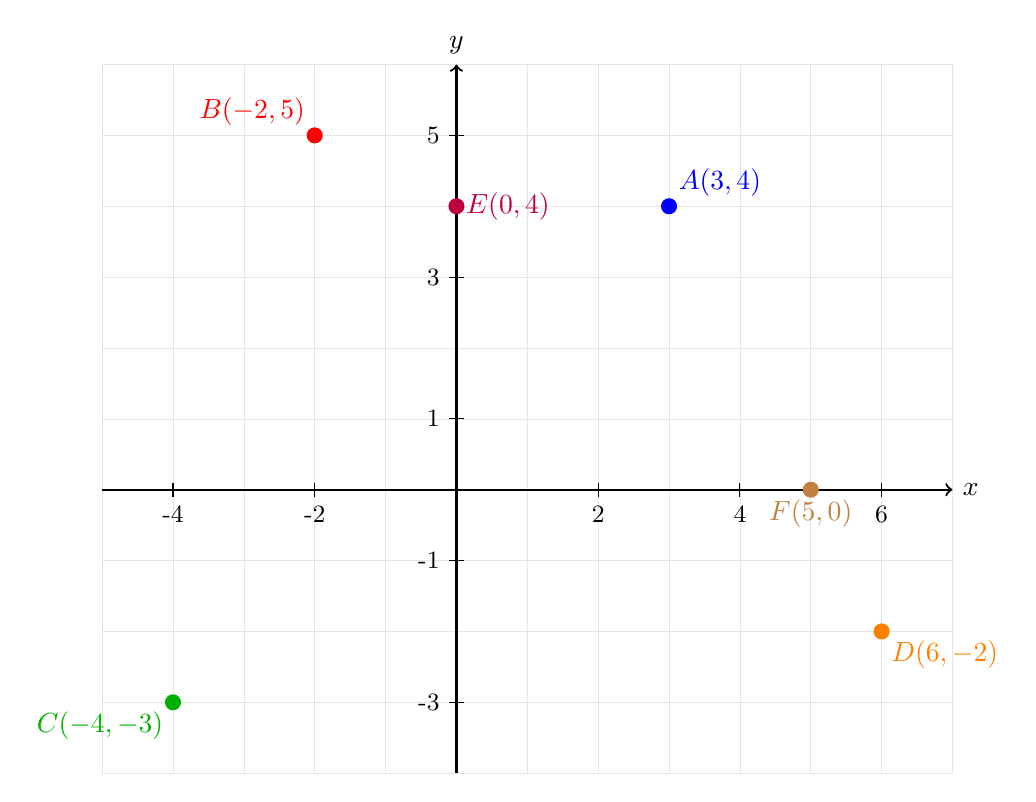
\begin{tikzpicture}[scale=0.9]
    % Grid
    \draw[gray!20, very thin] (-5,-4) grid (7,6);

    % Axes
    \draw[->, thick] (-5,0) -- (7,0) node[right] {$x$};
    \draw[->, thick] (0,-4) -- (0,6) node[above] {$y$};

    % Axis labels
    \foreach \x in {-4,-2,2,4,6}
        \draw (\x,0.1) -- (\x,-0.1) node[below, font=\small] {\x};
    \foreach \y in {-3,-1,1,3,5}
        \draw (0.1,\y) -- (-0.1,\y) node[left, font=\small] {\y};

    % Points
    \filldraw[blue] (3,4) circle (3pt);
    \node[blue, above right] at (3,4) {$A(3,4)$};

    \filldraw[red] (-2,5) circle (3pt);
    \node[red, above left] at (-2,5) {$B(-2,5)$};

    \filldraw[green!70!black] (-4,-3) circle (3pt);
    \node[green!70!black, below left] at (-4,-3) {$C(-4,-3)$};

    \filldraw[orange] (6,-2) circle (3pt);
    \node[orange, below right] at (6,-2) {$D(6,-2)$};

    \filldraw[purple] (0,4) circle (3pt);
    \node[purple, right] at (0,4) {$E(0,4)$};

    \filldraw[brown] (5,0) circle (3pt);
    \node[brown, below] at (5,0) {$F(5,0)$};
\end{tikzpicture}
\end{center}

\textbf{Observaciones:}
\begin{itemize}
    \item $A(3,4)$ está en el Cuadrante I
    \item $B(-2,5)$ está en el Cuadrante II
    \item $C(-4,-3)$ está en el Cuadrante III
    \item $D(6,-2)$ está en el Cuadrante IV
    \item $E(0,4)$ está sobre el eje $y$
    \item $F(5,0)$ está sobre el eje $x$
\end{itemize}

\newpage

\subsection*{Ejercicio 3: Cálculo de Distancias}

\textbf{Problema 1:} Distancia entre $(2, 5)$ y $(6, 8)$

Usando la fórmula de distancia:
\begin{align*}
d &= \sqrt{(x_2 - x_1)^2 + (y_2 - y_1)^2} \\
  &= \sqrt{(6 - 2)^2 + (8 - 5)^2} \\
  &= \sqrt{4^2 + 3^2} \\
  &= \sqrt{16 + 9} \\
  &= \sqrt{25} \\
  &= 5
\end{align*}

\textbf{Respuesta:} La distancia es 5 unidades.

\medskip

\textbf{Problema 2:} Distancia entre $(1, 3)$ y $(4, 7)$

\begin{align*}
d &= \sqrt{(4 - 1)^2 + (7 - 3)^2} \\
  &= \sqrt{3^2 + 4^2} \\
  &= \sqrt{9 + 16} \\
  &= \sqrt{25} \\
  &= 5
\end{align*}

\textbf{Respuesta:} La distancia es 5 unidades.

\medskip

\textbf{Problema 3:} Distancia entre $(-2, 1)$ y $(3, 4)$

\begin{align*}
d &= \sqrt{(3 - (-2))^2 + (4 - 1)^2} \\
  &= \sqrt{(3 + 2)^2 + 3^2} \\
  &= \sqrt{5^2 + 3^2} \\
  &= \sqrt{25 + 9} \\
  &= \sqrt{34} \\
  &\approx 5.83
\end{align*}

\textbf{Respuesta:} La distancia es $\sqrt{34} \approx 5.83$ unidades.

\medskip

\textbf{Problema 4:} Distancia entre $(-5, -2)$ y $(1, 6)$

\begin{align*}
d &= \sqrt{(1 - (-5))^2 + (6 - (-2))^2} \\
  &= \sqrt{6^2 + 8^2} \\
  &= \sqrt{36 + 64} \\
  &= \sqrt{100} \\
  &= 10
\end{align*}

\textbf{Respuesta:} La distancia es 10 unidades.

\medskip

\textbf{Problema 5:} Distancia entre $(0, 0)$ y $(3, 4)$

\begin{align*}
d &= \sqrt{(3 - 0)^2 + (4 - 0)^2} \\
  &= \sqrt{3^2 + 4^2} \\
  &= \sqrt{9 + 16} \\
  &= \sqrt{25} \\
  &= 5
\end{align*}

\textbf{Respuesta:} La distancia es 5 unidades.

\textbf{Nota:} Este es un triángulo rectángulo 3-4-5 clásico.

\medskip

\textbf{Problema 6:} Distancia entre $(-3, 7)$ y $(-3, -2)$

\begin{align*}
d &= \sqrt{(-3 - (-3))^2 + (-2 - 7)^2} \\
  &= \sqrt{0^2 + (-9)^2} \\
  &= \sqrt{0 + 81} \\
  &= \sqrt{81} \\
  &= 9
\end{align*}

\textbf{Respuesta:} La distancia es 9 unidades.

\textbf{Observación:} Como ambos puntos tienen la misma coordenada $x = -3$, están sobre una línea vertical. La distancia es simplemente la diferencia absoluta de las coordenadas $y$: $|7 - (-2)| = 9$.

\newpage

\subsection*{Ejercicio 4: Cálculo de Puntos Medios}

\textbf{Problema 1:} Punto medio entre $(4, 6)$ y $(8, 10)$

Usando la fórmula del punto medio:
\begin{align*}
M &= \left(\frac{x_1 + x_2}{2}, \frac{y_1 + y_2}{2}\right) \\
  &= \left(\frac{4 + 8}{2}, \frac{6 + 10}{2}\right) \\
  &= \left(\frac{12}{2}, \frac{16}{2}\right) \\
  &= (6, 8)
\end{align*}

\textbf{Respuesta:} El punto medio es $M(6, 8)$.

\medskip

\textbf{Problema 2:} Punto medio entre $(2, 3)$ y $(6, 9)$

\begin{align*}
M &= \left(\frac{2 + 6}{2}, \frac{3 + 9}{2}\right) \\
  &= \left(\frac{8}{2}, \frac{12}{2}\right) \\
  &= (4, 6)
\end{align*}

\textbf{Respuesta:} El punto medio es $M(4, 6)$.

\medskip

\textbf{Problema 3:} Punto medio entre $(-3, 5)$ y $(7, -1)$

\begin{align*}
M &= \left(\frac{-3 + 7}{2}, \frac{5 + (-1)}{2}\right) \\
  &= \left(\frac{4}{2}, \frac{4}{2}\right) \\
  &= (2, 2)
\end{align*}

\textbf{Respuesta:} El punto medio es $M(2, 2)$.

\medskip

\textbf{Problema 4:} Punto medio entre $(0, 0)$ y $(6, 8)$

\begin{align*}
M &= \left(\frac{0 + 6}{2}, \frac{0 + 8}{2}\right) \\
  &= \left(\frac{6}{2}, \frac{8}{2}\right) \\
  &= (3, 4)
\end{align*}

\textbf{Respuesta:} El punto medio es $M(3, 4)$.

\medskip

\textbf{Problema 5:} Punto medio entre $(-5, -3)$ y $(-1, 7)$

\begin{align*}
M &= \left(\frac{-5 + (-1)}{2}, \frac{-3 + 7}{2}\right) \\
  &= \left(\frac{-6}{2}, \frac{4}{2}\right) \\
  &= (-3, 2)
\end{align*}

\textbf{Respuesta:} El punto medio es $M(-3, 2)$.

\newpage

\subsection*{Ejercicio 5: Problemas Combinados}

\textbf{Problema 1:} Perímetro del triángulo con vértices $A(2, 1)$, $B(6, 3)$, y $C(4, 5)$

Calculamos la longitud de cada lado:

\textbf{Lado AB:}
\begin{align*}
d_{AB} &= \sqrt{(6-2)^2 + (3-1)^2} \\
       &= \sqrt{4^2 + 2^2} \\
       &= \sqrt{16 + 4} \\
       &= \sqrt{20} \\
       &= 2\sqrt{5}
\end{align*}

\textbf{Lado BC:}
\begin{align*}
d_{BC} &= \sqrt{(4-6)^2 + (5-3)^2} \\
       &= \sqrt{(-2)^2 + 2^2} \\
       &= \sqrt{4 + 4} \\
       &= \sqrt{8} \\
       &= 2\sqrt{2}
\end{align*}

\textbf{Lado AC:}
\begin{align*}
d_{AC} &= \sqrt{(4-2)^2 + (5-1)^2} \\
       &= \sqrt{2^2 + 4^2} \\
       &= \sqrt{4 + 16} \\
       &= \sqrt{20} \\
       &= 2\sqrt{5}
\end{align*}

\textbf{Perímetro:}
\begin{align*}
P &= d_{AB} + d_{BC} + d_{AC} \\
  &= 2\sqrt{5} + 2\sqrt{2} + 2\sqrt{5} \\
  &= 4\sqrt{5} + 2\sqrt{2} \\
  &\approx 4(2.236) + 2(1.414) \\
  &\approx 8.944 + 2.828 \\
  &\approx 11.77
\end{align*}

\textbf{Respuesta:} El perímetro es $4\sqrt{5} + 2\sqrt{2} \approx 11.77$ unidades.

\textbf{Nota:} El triángulo es isósceles porque $d_{AB} = d_{AC}$.

\medskip

\textbf{Problema 2:} Punto medio entre $(5, -3)$ y $(-1, 7)$, luego distancia desde el origen

\textbf{Paso 1:} Encontrar el punto medio
\begin{align*}
M &= \left(\frac{5 + (-1)}{2}, \frac{-3 + 7}{2}\right) \\
  &= \left(\frac{4}{2}, \frac{4}{2}\right) \\
  &= (2, 2)
\end{align*}

\textbf{Paso 2:} Calcular distancia del origen $(0, 0)$ al punto medio $(2, 2)$
\begin{align*}
d &= \sqrt{(2-0)^2 + (2-0)^2} \\
  &= \sqrt{4 + 4} \\
  &= \sqrt{8} \\
  &= 2\sqrt{2} \\
  &\approx 2.83
\end{align*}

\textbf{Respuesta:} El punto medio es $(2, 2)$ y su distancia al origen es $2\sqrt{2} \approx 2.83$ unidades.

\medskip

\textbf{Problema 3:} ¿Es isósceles el triángulo con vértices $A(0, 0)$, $B(3, 4)$, y $C(6, 0)$?

Calculamos las tres longitudes:

\textbf{Lado AB:}
$$d_{AB} = \sqrt{(3-0)^2 + (4-0)^2} = \sqrt{9 + 16} = \sqrt{25} = 5$$

\textbf{Lado BC:}
$$d_{BC} = \sqrt{(6-3)^2 + (0-4)^2} = \sqrt{9 + 16} = \sqrt{25} = 5$$

\textbf{Lado AC:}
$$d_{AC} = \sqrt{(6-0)^2 + (0-0)^2} = \sqrt{36} = 6$$

Como $d_{AB} = d_{BC} = 5$ (dos lados iguales), el triángulo \textbf{SÍ es isósceles}.

\textbf{Respuesta:} Sí, el triángulo es isósceles con dos lados de longitud 5 unidades.

\newpage

\subsection*{Ejercicio 6: Problemas de Aplicación}

\textbf{Problema 1:} Distancia entre biblioteca $(3, 5)$ y parque $(9, 13)$ en kilómetros

\begin{align*}
d &= \sqrt{(9-3)^2 + (13-5)^2} \\
  &= \sqrt{6^2 + 8^2} \\
  &= \sqrt{36 + 64} \\
  &= \sqrt{100} \\
  &= 10
\end{align*}

\textbf{Respuesta:} La distancia entre la biblioteca y el parque es 10 kilómetros.

\textbf{Observación:} Este es un triángulo rectángulo 6-8-10, que es el doble del triángulo clásico 3-4-5.

\medskip

\textbf{Problema 2:} Posición del barco a mitad del camino entre $A(-4, 2)$ y $B(8, 7)$

El punto medio representa la mitad del camino:
\begin{align*}
M &= \left(\frac{-4 + 8}{2}, \frac{2 + 7}{2}\right) \\
  &= \left(\frac{4}{2}, \frac{9}{2}\right) \\
  &= \left(2, 4.5\right)
\end{align*}

\textbf{Respuesta:} El barco se encuentra en el punto $(2, 4.5)$.

\textbf{Verificación opcional:} Podemos verificar que las distancias $d(A,M)$ y $d(M,B)$ son iguales.

\medskip

\textbf{Problema 3:} ¿Es equilátero el triángulo con vértices $A(0, 0)$, $B(12, 0)$, y $C(6, 8)$?

\textbf{Lado AB:}
$$d_{AB} = \sqrt{(12-0)^2 + (0-0)^2} = \sqrt{144} = 12$$

\textbf{Lado AC:}
$$d_{AC} = \sqrt{(6-0)^2 + (8-0)^2} = \sqrt{36 + 64} = \sqrt{100} = 10$$

\textbf{Lado BC:}
$$d_{BC} = \sqrt{(6-12)^2 + (8-0)^2} = \sqrt{36 + 64} = \sqrt{100} = 10$$

Como los tres lados no son iguales ($12 \neq 10$), el triángulo \textbf{NO es equilátero}.

Sin embargo, como $d_{AC} = d_{BC} = 10$, el triángulo \textbf{SÍ es isósceles}.

\textbf{Respuesta:} El triángulo NO es equilátero, pero SÍ es isósceles con dos lados de 10 unidades y una base de 12 unidades.

\newpage

\subsection*{Ejercicio 7: Problemas Desafiantes}

\textbf{Problema 1:} Encontrar extremo $B$ dado punto medio $M(4, 3)$ y extremo $A(2, 7)$

Sea $B(x, y)$ el extremo desconocido. Usamos la fórmula del punto medio:

$$M = \left(\frac{x_1 + x}{2}, \frac{y_1 + y}{2}\right) = (4, 3)$$

\textbf{Para la coordenada $x$:}
\begin{align*}
\frac{2 + x}{2} &= 4 \\
2 + x &= 8 \\
x &= 6
\end{align*}

\textbf{Para la coordenada $y$:}
\begin{align*}
\frac{7 + y}{2} &= 3 \\
7 + y &= 6 \\
y &= -1
\end{align*}

\textbf{Respuesta:} El otro extremo es $B(6, -1)$.

\textbf{Verificación:}
$$M = \left(\frac{2 + 6}{2}, \frac{7 + (-1)}{2}\right) = \left(\frac{8}{2}, \frac{6}{2}\right) = (4, 3)$$ \checkmark

\medskip

\textbf{Problema 2:} Demostrar que $A(1, 2)$, $B(3, 6)$, $C(5, 10)$ son colineales

Tres puntos son colineales si y solo si $d(A,B) + d(B,C) = d(A,C)$.

\textbf{Distancia AB:}
\begin{align*}
d_{AB} &= \sqrt{(3-1)^2 + (6-2)^2} \\
       &= \sqrt{4 + 16} \\
       &= \sqrt{20} \\
       &= 2\sqrt{5}
\end{align*}

\textbf{Distancia BC:}
\begin{align*}
d_{BC} &= \sqrt{(5-3)^2 + (10-6)^2} \\
       &= \sqrt{4 + 16} \\
       &= \sqrt{20} \\
       &= 2\sqrt{5}
\end{align*}

\textbf{Distancia AC:}
\begin{align*}
d_{AC} &= \sqrt{(5-1)^2 + (10-2)^2} \\
       &= \sqrt{16 + 64} \\
       &= \sqrt{80} \\
       &= 4\sqrt{5}
\end{align*}

\textbf{Verificación:}
$$d_{AB} + d_{BC} = 2\sqrt{5} + 2\sqrt{5} = 4\sqrt{5} = d_{AC}$$ \checkmark

Como se cumple la condición, los tres puntos \textbf{SON colineales}.

\textbf{Método alternativo:} También podemos verificar que la pendiente entre $A$ y $B$ es igual a la pendiente entre $B$ y $C$:
$$m_{AB} = \frac{6-2}{3-1} = \frac{4}{2} = 2$$
$$m_{BC} = \frac{10-6}{5-3} = \frac{4}{2} = 2$$

Como las pendientes son iguales, los puntos están sobre la misma recta.

\medskip

\textbf{Problema 3:} Longitud de las diagonales del rectángulo con vértices $A(1, 1)$, $B(5, 1)$, $C(5, 4)$, $D(1, 4)$

Las diagonales de un rectángulo son $\overline{AC}$ y $\overline{BD}$.

\textbf{Diagonal AC:}
\begin{align*}
d_{AC} &= \sqrt{(5-1)^2 + (4-1)^2} \\
       &= \sqrt{16 + 9} \\
       &= \sqrt{25} \\
       &= 5
\end{align*}

\textbf{Diagonal BD:}
\begin{align*}
d_{BD} &= \sqrt{(1-5)^2 + (4-1)^2} \\
       &= \sqrt{16 + 9} \\
       &= \sqrt{25} \\
       &= 5
\end{align*}

\textbf{Respuesta:} Ambas diagonales miden 5 unidades.

\textbf{Verificación:} En un rectángulo, las diagonales siempre tienen la misma longitud, lo cual se confirma aquí. Además, podemos verificar que es un rectángulo calculando los lados:
\begin{itemize}
    \item $d_{AB} = 4$ (lado horizontal)
    \item $d_{BC} = 3$ (lado vertical)
    \item $d_{CD} = 4$ (lado horizontal)
    \item $d_{DA} = 3$ (lado vertical)
\end{itemize}

Los lados opuestos son iguales, confirmando que es un rectángulo.

\newpage

\subsection*{Ejercicio 8: Práctica Mixta}

\textbf{a)} Punto medio entre $(7, 11)$ y $(3, 5)$

$$M = \left(\frac{7+3}{2}, \frac{11+5}{2}\right) = \left(\frac{10}{2}, \frac{16}{2}\right) = (5, 8)$$

\medskip

\textbf{b)} Distancia entre $(-6, 2)$ y $(2, 8)$

\begin{align*}
d &= \sqrt{(2-(-6))^2 + (8-2)^2} \\
  &= \sqrt{8^2 + 6^2} \\
  &= \sqrt{64 + 36} \\
  &= \sqrt{100} \\
  &= 10
\end{align*}

\medskip

\textbf{c)} Encontrar el otro extremo si $M(5, 3)$ es punto medio y un extremo es $(8, 7)$

Sea $B(x, y)$ el otro extremo:

Para $x$: $\dfrac{8 + x}{2} = 5 \implies 8 + x = 10 \implies x = 2$

Para $y$: $\dfrac{7 + y}{2} = 3 \implies 7 + y = 6 \implies y = -1$

El otro extremo es $B(2, -1)$.

\medskip

\textbf{d)} ¿Es rectángulo el triángulo con vértices $(0, 0)$, $(5, 0)$, y $(0, 12)$?

Calculamos las tres distancias:
$$d_{AB} = \sqrt{5^2 + 0^2} = 5$$
$$d_{BC} = \sqrt{5^2 + 12^2} = \sqrt{25 + 144} = \sqrt{169} = 13$$
$$d_{AC} = \sqrt{0^2 + 12^2} = 12$$

Verificamos el teorema de Pitágoras:
$$5^2 + 12^2 = 25 + 144 = 169 = 13^2$$ \checkmark

\textbf{Sí, es un triángulo rectángulo} con el ángulo recto en el origen.

\medskip

\textbf{e)} Perímetro del cuadrilátero con vértices $A(0, 0)$, $B(4, 0)$, $C(4, 3)$, $D(0, 3)$

Este es un rectángulo con base 4 y altura 3.

$$P = 2(\text{base}) + 2(\text{altura}) = 2(4) + 2(3) = 8 + 6 = 14$$

\textbf{Respuesta:} El perímetro es 14 unidades.

\textbf{Verificación calculando cada lado:}
\begin{itemize}
    \item $d_{AB} = 4$
    \item $d_{BC} = 3$
    \item $d_{CD} = 4$
    \item $d_{DA} = 3$
    \item Perímetro = $4 + 3 + 4 + 3 = 14$ \checkmark
\end{itemize}
